
\begin{problem}[习题2.8]
考虑下面这棵假想的对策树:
\begin{center}
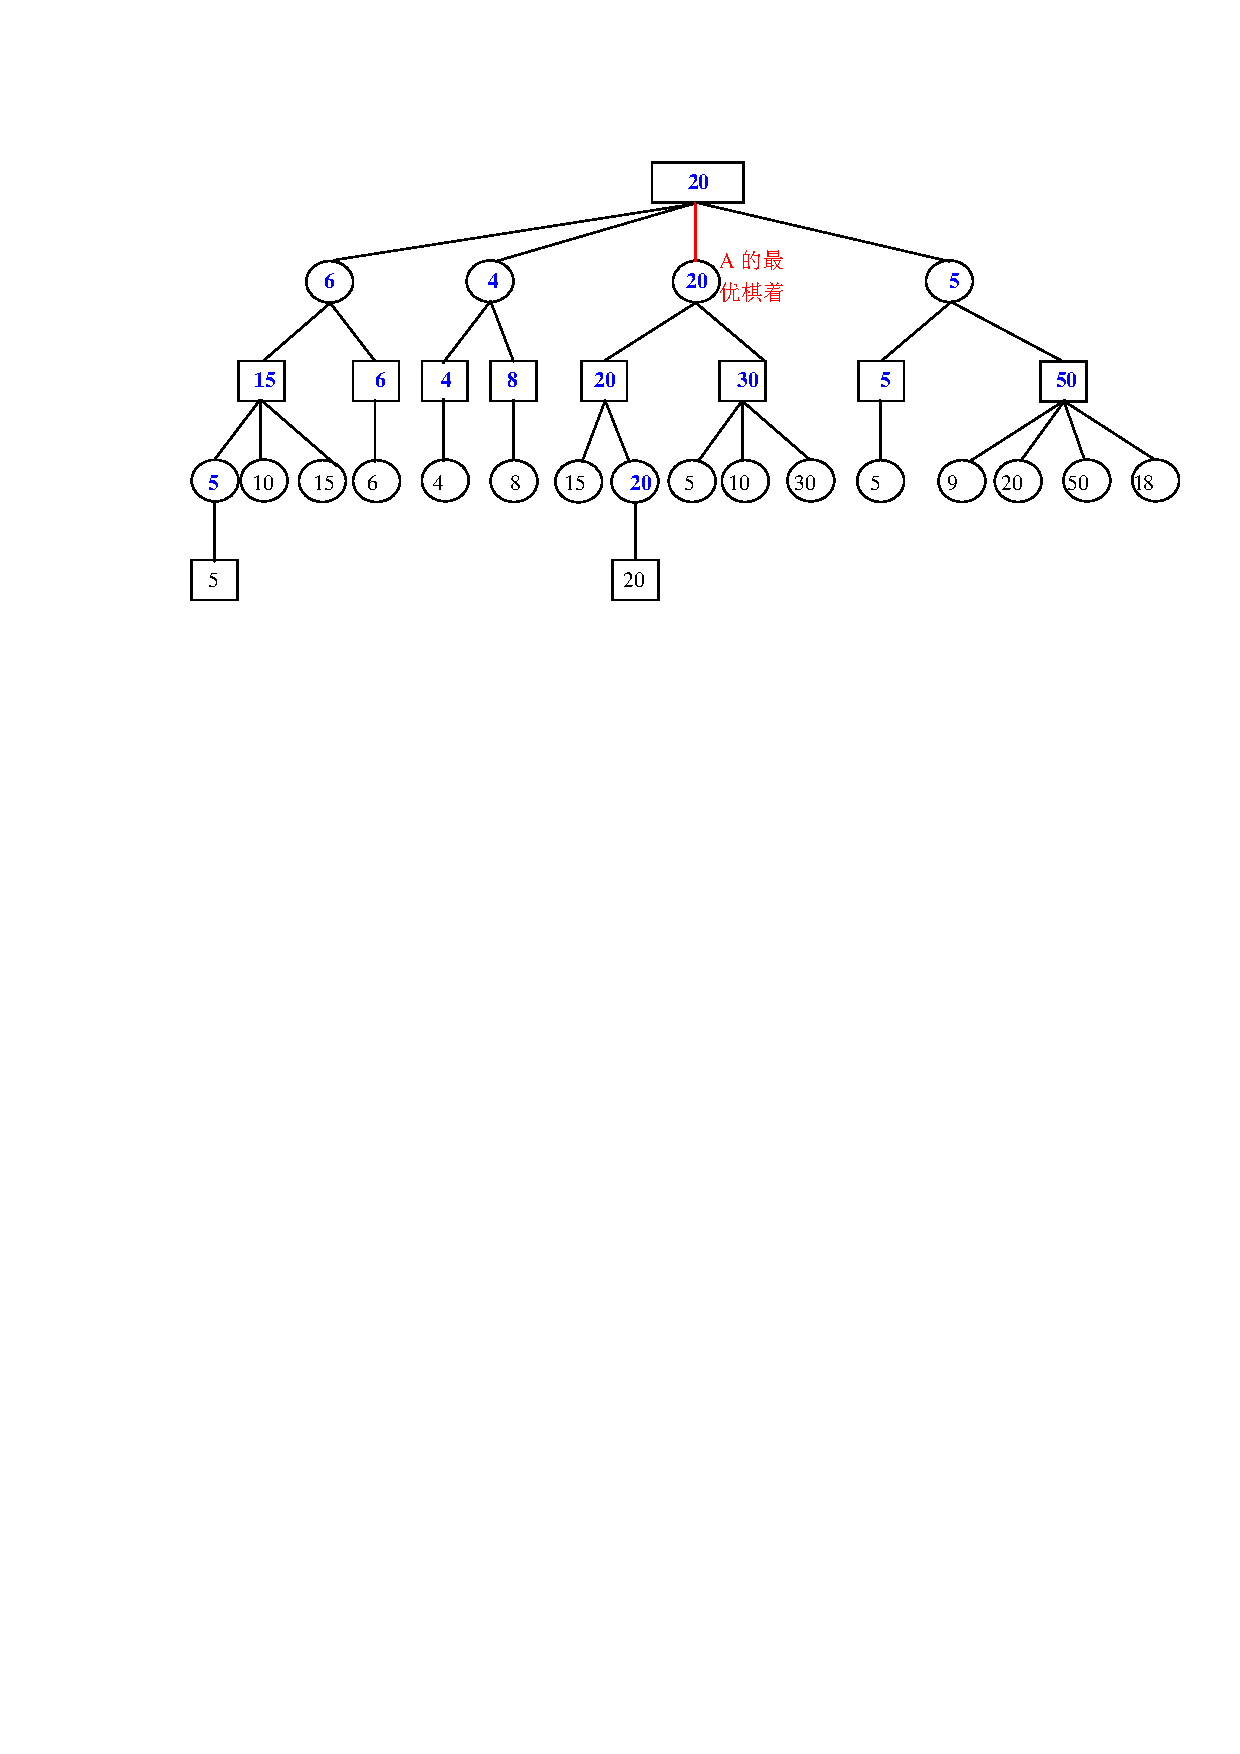
\includegraphics[width=0.8\textwidth]{fig02.pdf}\\
\end{center}
\begin{enumerate}
\item 使用最大最小方法(2-4-2)式获取各结点的值;
\item 弈者$A$为获胜应该什么棋着?
\item 列出算法$VEB$计算这棵对策树结点的值时各结点被计算的顺序;
\item 对树中每个结点$X$,用(2-4-3)式计算$V(X)$;
\item 在取$X=\textrm{根}$,$l=10$, $LB=-\infty$, $D=\infty$的情况下, 用算法$AB$计算此树的根的值期间, 这棵树的那些结点没有计算?
\end{enumerate}
\end{problem}
\begin{solution}
\begin{enumerate}
\item 各结点的值已在题中所给图中标出;
\item 弈者$A$为获胜应该走的棋着已在题中所给图中标出;
\item 算法$VEB$计算这棵对策树结点的值时各结点被计算的顺序如图\ref{ans34}中的红色数字;
\item 对树中每个结点$X$,用(2-4-3)式计算$V(X)$所得的值,已标在图\ref{ans34}中的方框或圆圈中(蓝色数字);
\begin{figure}[!htb]
\centering
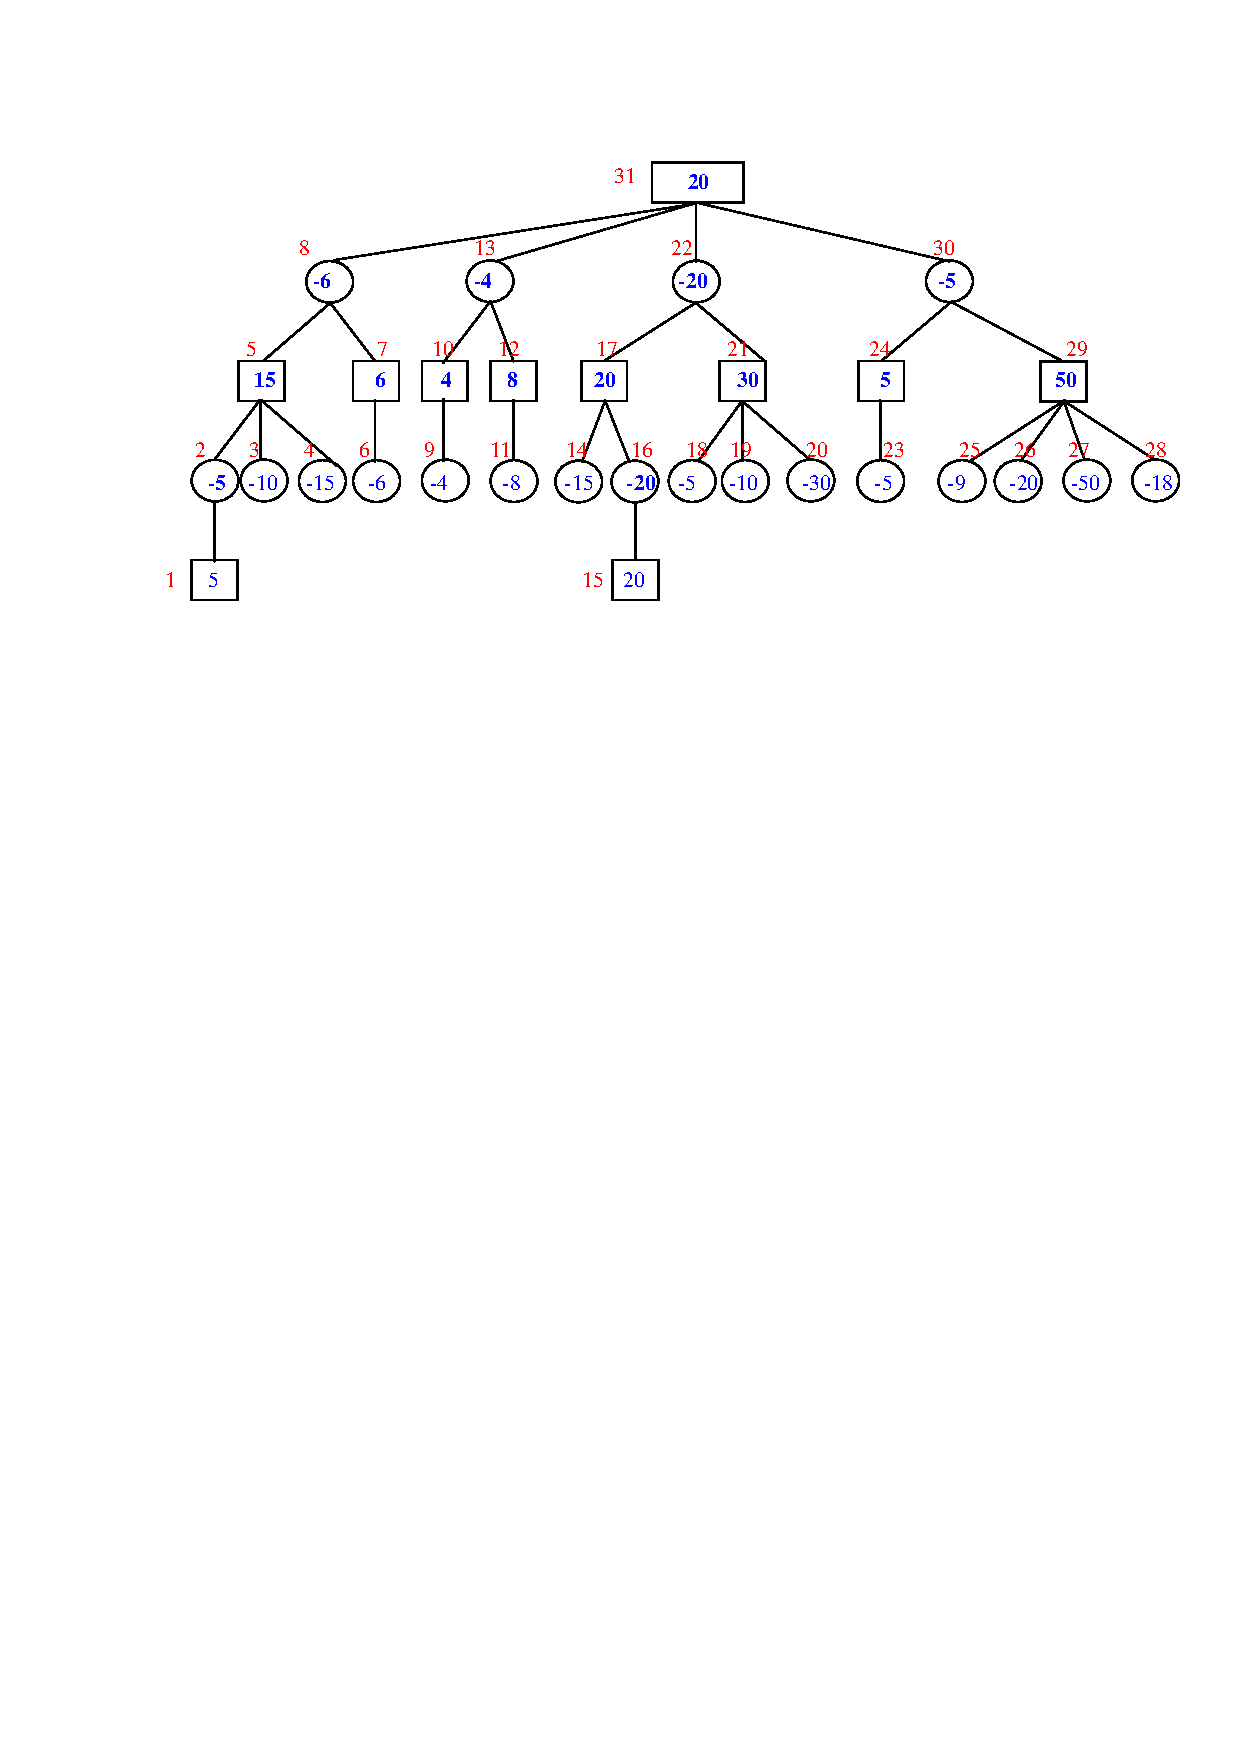
\includegraphics[width=0.8\textwidth]{fig02_1.pdf}
\caption{\label{ans34}第(3)(4)小问解}
\end{figure}
\item 在取$X=\textrm{根}$,$l=10$, $LB=-\infty$, $D=\infty$的情况下, 图\ref{ans34}中标有以下红色数字中的结点没有被计算:
    \[
    11, 12, 25, 26, 27, 28, 29
    \]
\end{enumerate}
\end{solution}
